\documentclass[12pt]{article}

\usepackage[T1]{fontenc}
\usepackage[utf8]{inputenc}
\usepackage{mathpazo}
\usepackage[margin=1in]{geometry}
\usepackage{setspace}
\setstretch{2.0}
\usepackage{amsmath,amssymb,amsthm}
\usepackage{booktabs}
\usepackage{graphicx}
\usepackage{float}
\usepackage[bottom]{footmisc}
\usepackage[authoryear]{natbib}
\usepackage{url}
\usepackage{hyperref}
\hypersetup{colorlinks=true,linkcolor=black,citecolor=black,urlcolor=blue}

\title{The Asymmetric Timeliness of Earnings Revisited: \\
A Replication of \citet{basu1997} on U.S. Firms, 2015--2024}
\author{Justin Cheng \\ University of Oklahoma}
\date{May 2026}

\begin{document}
\maketitle

\begin{abstract}
\noindent
\citet{basu1997} found that accounting earnings react faster to bad economic news than to good news, and read the result as evidence of conditional conservatism. I take his test to a fresh decade on a sample of 17{,}188 firm-years from the Compustat--CRSP merged universe of U.S. listed non-financial firms with December fiscal year-ends running 2015 through 2024, with standard errors clustered by firm throughout. The asymmetric-timeliness coefficient $\beta_3$ comes in at $0.402$ ($t=26.4$) in the pooled sample, so the underlying property still seems to be there in the modern data. The pre-COVID sub-sample average ($0.450$) sits a touch above the COVID-era average ($0.364$), which on its own would look like mild compression, but the year-by-year path is not monotonic at all. $\beta_3$ jumps to $0.598$ in fiscal 2020 before collapsing to $0.134$ in 2021 and drifting back to its historical band over the three years that follow. I read the 2020 spike as consistent with the impairment-heavy COVID onset and the 2021 collapse as the recovery year, when the same firms whose returns had flipped positive could not easily reverse their prior write-downs. The model is reduced-form, not causal: I do not argue that COVID itself drove the V. The coefficient still picks up the relative loading of earnings on bad-return news versus good-return news, the mechanic that conservatism is supposed to generate, so single-year readings carry wide bars and should not be over-read, but the year-by-year path remains useful as a trend signal.
\end{abstract}

\section{Introduction}
The accounting literature has long held that gains demand more verifiable evidence than losses, and that this asymmetry pushes accountants to book bad news into earnings sooner than good news \citep{watts2003a, watts2003b}. \citet{basu1997} turned that idea into an empirical test by running a reverse regression of earnings on contemporaneous returns, where a positive coefficient on the return-times-bad-news interaction reads as evidence of conditional conservatism.

The Basu test went on to become the standard design in the conservatism literature, though the original sample ran only from 1963 to 1990. A fair amount of subsequent work has questioned whether the asymmetry survives in more recent decades, especially after the post-1990 fair-value rules and the broader move from reliability toward relevance reshaped GAAP. \citet{dietrich2007} push the critique furthest, arguing that several mechanical features of the regression generate a positive interaction even when no real conservatism is present in the underlying accounting choice. The open question on the table for this paper is whether $\beta_3$ still comes in big and positive when the test is rerun on the post-2015 panel.

I revisit the test on fiscal years 2015--2024 using the WRDS Compustat--CRSP merged universe, with the paper falling into two pieces. The first piece is an out-of-sample replication of the original test on the most recent ten-year window, which speaks directly to the debate over whether modern accounting standards have eroded the asymmetry, while the second pulls in the COVID-19 shock as a natural high-uncertainty episode and asks how $\beta_3$ moved through 2020--2024.

The empirical strategy hews close to \citet{basu1997}. Earnings scaled by beginning-of-period price are regressed on the fiscal-year return, a bad-news indicator, and their interaction. The coefficient $\beta_3$ on the interaction is the parameter of interest, and the conservatism hypothesis predicts $\beta_3>0$. I make two adjustments to the 1997 design. Following \citet{petersen2009}, standard errors are clustered at the firm level rather than left at OLS defaults. And, again following the banking-conservatism convention, financial firms (SIC 6000--6999) are dropped, because their loan-loss, securities, and insurance accounting blends mark-to-market with historical-cost in ways that distort earnings comparability.

Pooled across 2015--2024, $\hat{\beta}_3 = 0.402$ ($t=26.4$). That is in the same neighborhood as the $\sim 0.35$ Basu reported for 1963--1990. Splitting the panel into a pre-COVID block (2015--2019) and a COVID-era block (2020--2024) gives $\hat{\beta}_3 = 0.450$ and $0.364$, which read as mild compression. The year-by-year coefficients tell a different story. From $0.46$ in 2019 the coefficient leaps to $0.60$ in 2020, falls to $0.13$ in 2021, then climbs back through $0.31$, $0.57$, and $0.52$ in 2022, 2023, and 2024. I read this V as the imprint of the COVID shock on the cross-section of bad-news firms, filtered through the one-sided impairment rules in U.S. GAAP.

Section~\ref{sec:literature} sets up the conservatism literature: the original Basu test, the Watts surveys, the firm-year extension of \citet{khan2009}, and the Dietrich--Muller--Riedl critique. Section~\ref{sec:data} describes the WRDS pull and the sample-construction choices. Section~\ref{sec:methods} writes out the specification and the standard-error structure. Section~\ref{sec:findings} reports pooled, sub-sample, and year-by-year results. Section~\ref{sec:conclusion} closes.

\section{Literature Review}
\label{sec:literature}
\citet{basu1997} treated the year's stock return as a noisy proxy for news about the firm. Positive returns capture good news that may or may not yet be reflected in earnings. Negative returns capture losses that are usually verified and so have to be booked. From those two observations follows the prediction the test exploits: the slope of earnings on returns should be steeper when returns are negative. The Basu regression captures the steepening with one interaction term.

\citet{watts2003a} and \citet{watts2003b} survey the theoretical motivations for conservatism. Contracting demands, litigation exposure, tax planning, and political-cost incentives each push managers to defer the recognition of unverified gains. Watts also reviews the early empirical work and lays out the family of tests, of which the Basu reverse regression is one.

\citet{ball2005} take the Basu test to U.K. private firms and show that contracting and debt-market demands sharpen loss-recognition timeliness in publicly held firms. \citet{khan2009} construct a firm-year conservatism score, $\mathit{C\_Score}$, by parameterizing the Basu coefficients on size, leverage, and market-to-book, then document substantial cross-sectional variation. \citet{lawrence2013} flag a mechanical concern: part of the asymmetry could come from non-discretionary GAAP rules, like impairment, rather than from any deliberate conservatism in accounting choice.

The methodological critique of \citet{dietrich2007} is the most aggressive of those in the literature. They argue that several features of the standard test inflate $\beta_3$, including a sample-selection problem that arises when returns are truncated and a mechanical correlation that shows up whenever earnings and returns share the same denominator. The remedies they recommend are firm-clustered standard errors and explicit subsample reporting, both of which I adopt in what follows. \citet{ruch2015} review the post-Dietrich literature and conclude that the basic Basu coefficient still works as a descriptive statistic for cross-sectional and time-series comparisons, even if its interpretation has narrowed since the original test was written down.

A separate strand of work asks how conservatism varies with the firm's information and contracting environment. \citet{khan2009} find that smaller and more leveraged firms with higher growth prospects book earnings more conservatively, and the firm-year score they construct has since been used widely as a conditioning variable in the cross-section. Several panel studies document a secular decline in conservatism through the 1990s and 2000s, attributing the drift to the shift in standard-setting from reliability toward relevance together with the spread of fair-value measurement under SFAS 157. \citet{lawrence2013} push back along a related line: a substantial share of the measured asymmetry is non-discretionary GAAP machinery rather than a contracting choice, so part of the secular drift in $\beta_3$ may reflect tightening of impairment rules rather than any deeper shift in conservatism preferences.

One piece of the modern conservatism story tends to get glossed over in the Basu literature, which is the role of the GAAP impairment rules themselves. Goodwill impairment under SFAS 142 (now ASC 350) and long-lived asset impairment under SFAS 144 (now ASC 360) are both one-sided in the direction the Basu test cares about. Under SFAS 142 a firm tests goodwill for impairment at least annually and writes it down when carrying value exceeds fair value, and once a write-down has gone through, the value cannot be written back up under U.S. GAAP even if the underlying business later recovers. SFAS 144 then follows the same one-sided asymmetry for property, plant, and equipment held for use. The accounting therefore takes the losses without taking the corresponding gains, which is exactly the loss-recognition timeliness the Basu coefficient is designed to detect. Two consequences for the year-by-year exercise in Section~\ref{sec:findings} fall out of this rule structure. The first is that in any year in which a non-trivial fraction of firms triggers impairment, $\beta_3$ ought to rise mechanically, regardless of any change in the underlying contracting or litigation incentives. A related consequence is that in the year immediately after a wave of impairments, the same firms cannot reverse those losses even if their economic prospects flip, so the bad-news slope $\beta_2 + \beta_3$ should fall in that subsequent year. The second of these predictions is what becomes important for interpreting the 2020--2021 swing in particular.

The 2008--2009 financial crisis offers a useful template for the COVID-era exercise here. Several papers report that the Basu coefficient rose sharply in 2008 as banks and insurers along with leveraged non-financials booked large impairments, before falling back in 2009 and 2010 as conditions normalized. I have not found published work that traces the analogous pattern around COVID-19 on the modern Compustat--CRSP universe, and filling in that gap is what this paper sets out to do.

\section{Data}
\label{sec:data}
The firm-year observations come from the WRDS Compustat--CRSP merged universe over fiscal years 2014--2025, with the 2014 vintage used only to construct lagged prices for the 2015 observations. From the \texttt{comp.funda} table I pull earnings per share excluding extraordinary items ($\mathit{epspx}$) together with the fiscal-year-end share price ($\mathit{prcc\_f}$) and the cumulative split-adjustment factor ($\mathit{ajex}$). Monthly stock returns come from \texttt{crsp.msf}, with the two universes linked through \texttt{crsp.ccmxpf\_lnkhist}.

Sample filters here are conventional in the literature. I keep U.S. common stocks (CRSP \texttt{shrcd} $\in \{10, 11\}$) traded on NYSE, AMEX, or NASDAQ, with December fiscal year-ends and a beginning-of-period price above one dollar, and I require earnings, prices, and returns all to be non-missing. Financial firms (SIC 6000--6999) are dropped, again following the banking-conservatism literature.

The fiscal-year stock return $R_{it}$ is the compounded return on firm $i$ over the twelve calendar months ending in fiscal year-end month $t$. I require returns to be present for all twelve months, which removes firms that delisted mid-year or that had not yet started trading at the start of the fiscal year. Following \citet{basu1997}, scaled earnings are
\[
EP_{it} = \frac{\mathit{epspx}_{it}}{\mathit{prcc\_f}_{i,t-1} \cdot \mathit{ajex}_{it}/\mathit{ajex}_{i,t-1}},
\]
that is, EPS divided by the split-adjusted beginning-of-period price. Without the split adjustment the denominator can shift discontinuously when a firm splits its stock during the year, which would inject pure mechanical noise into $EP$. Both $EP$ and $R$ are winsorized at the 1\% and 99\% pooled tails to limit the leverage of extreme observations. This is standard practice in the conservatism literature.

The merge between Compustat and CRSP runs through \texttt{ccmxpf\_lnkhist}. I retain links of type \texttt{LU} (untested but credible) or \texttt{LC} (researcher-confirmed) with primary or co-primary status, the conservative standard recommended by WRDS. The fiscal-year-end date must fall inside both the link's effective window (\texttt{linkdt} to \texttt{linkenddt}) and the CRSP names-history window (\texttt{namedt} to \texttt{nameenddt}), so that the share-code and exchange filters apply to the version of the security trading at the actual fiscal year-end.

After all filters the analysis sample contains 17{,}188 firm-years from 3{,}167 unique firms over fiscal years 2015--2024. Fiscal 2025 is too sparse in Compustat at the time of writing and so falls out of the analysis window even though it sits inside the WRDS pull range. Table~\ref{tab:desc} reports descriptive statistics on the four key variables. Table~\ref{tab:yearly_n} breaks the sample down by fiscal year and reports the share of bad-news firm-years. The bad-news share moves between roughly 31\% and 73\%, with the highest readings in 2018 (66\%) and 2022 (73\%), the two years in which the broad market indices posted negative annual returns over my sample.

\section{Methods}
\label{sec:methods}
The estimating equation is the canonical \citet{basu1997} reverse regression
\begin{equation}
  EP_{it} \;=\; \beta_{0} + \beta_{1}D_{it} + \beta_{2}R_{it}
        + \beta_{3} D_{it} R_{it} + \varepsilon_{it},
  \label{eq:basu}
\end{equation}
where $D_{it} = \mathbf{1}\{R_{it} < 0\}$ is the bad-news dummy. $\beta_{2}$ is the sensitivity of earnings to good news, and $\beta_{2} + \beta_{3}$ is the sensitivity to bad news. The interaction coefficient $\beta_{3}$ is the parameter of interest. Conditional conservatism predicts $\beta_{3} > 0$.

I estimate equation~\eqref{eq:basu} by OLS with heteroskedasticity-robust standard errors clustered at the firm level \citep{petersen2009}. Firm-level clustering matters here. The same firm contributes up to ten observations to the panel, and within-firm errors are likely to be serially correlated. I do not also cluster on year. Ten year clusters is too few for the asymptotics to bite, and adding the second dimension would push the specification away from the original Basu test for very little gain.

To gauge the stability of the coefficient over time I re-estimate the model on the pre-COVID block (fiscal 2015--2019) and the COVID-era block (2020--2024), and I also estimate equation~\eqref{eq:basu} year by year. The year-by-year regressions necessarily lean on the 1{,}600--1{,}900 observations available in each fiscal year, so the standard errors are wider. Figure~\ref{fig:beta3} reports 95\% confidence bars on those point estimates, so the reader can judge how much of the year-to-year movement could be sampling noise alone.

I do not include firm or year fixed effects in the baseline specification. With firm fixed effects in the regression, almost all of the cross-sectional variation in $EP$ and $R$ gets soaked up, and the interaction ends up identified off within-firm changes in the sign of news only, which is not what the Basu test is trying to pin down. Year fixed effects are a different case. They absorb the average level of $EP$ year-by-year but, because $D \times R$ already moves around within any given year by construction, they leave $\beta_3$ where it was.

Two measurement choices in particular deserve direct comment, since both materially affect the headline coefficient. The winsorization rule is the first of them. EPS scaled by lagged price carries a fat right tail driven by firms with extremely small base-period prices, so the simple OLS fit can get pulled around by a handful of $EP$ observations sitting up at three or four. I follow the post-Basu convention here and winsorize $EP$ and $R$ at the pooled 1\% and 99\% tails, which keeps every observation in the panel but caps the influence of the extreme ones; outright trimming would have been the alternative. Trimming would drop small-price firms from the sample entirely. Those firms are exactly the population in which conservatism shows up most strongly, and dropping them would attenuate $\beta_3$. Standard errors are the second of the two choices. Firm-clustered errors are what \citet{petersen2009} recommends for samples with many firms but few years, and the present panel falls squarely in that category. The natural alternative is a two-way firm-and-year cluster, which on paper would be more conservative, but ten year clusters sits well below the 30--50 rule of thumb that Cameron--Gelbach--Miller asymptotics need to bite, and the resulting standard errors would come out unreliable rather than larger. Driscoll--Kraay errors, which are designed for short panels with cross-sectional dependence, would handle that issue but at the cost of reporting a coefficient that no other paper in this literature has used. I keep firm-clustered errors here and flag the two-way cluster as a robustness extension. Neither choice changes the sign or significance of the asymmetric-timeliness coefficient.

\section{Findings}
\label{sec:findings}
Table~\ref{tab:basu} reports OLS estimates of equation~\eqref{eq:basu}. In the pooled sample the good-news slope $\beta_{2} = -0.080$ ($t=-10.5$) is small in absolute value but tightly estimated. The asymmetric-timeliness coefficient $\beta_{3} = 0.402$ ($t=26.4$) is large, positive, and very tightly estimated. The implied bad-news slope is $\beta_{2} + \beta_{3} = 0.323$, while the good-news slope $\beta_{2}$ is near zero and actually slightly negative; the bad-news slope is therefore about four times as large in absolute value. That is the same qualitative gap \citet{basu1997} found for 1963--1990: earnings load on bad-return news much faster than on good-return news.

The pre-/post-COVID comparison shows the coefficient slightly lower in the COVID era ($\beta_{3} = 0.364$) than in the pre-COVID block ($\beta_{3} = 0.450$). Taken at face value the gap looks like mild compression. The two-period average, however, hides a much sharper pattern. Figure~\ref{fig:beta3} traces the year-by-year coefficient with 95\% bars. From $0.46$ in 2019 the point estimate jumps to $0.60$ in 2020, the COVID-19 onset, then collapses to $0.13$ in 2021 before climbing back to $0.31$, $0.57$, and $0.52$ in 2022 through 2024. The regression is reduced-form. It is not a causal model, and I do not claim that the COVID shock itself caused $\beta_3$ to swing. What the coefficient does capture is the relative loading of earnings on bad-return news versus good-return news, which is exactly the mechanic conservatism is supposed to generate. Single-year point estimates carry wide confidence bars, so no one year should be over-read on its own. The V itself, though, sits well outside anything sampling noise alone would produce, and the year-to-year swings remain informative as a coarse trend reading.

I read the V as a mechanical consequence of how the Basu test interacts with macroeconomic shocks. In 2020 a large fraction of firms realized genuinely bad news ($D_{it} = 1$). Impairments, restructurings, and going-concern adjustments all hit earnings hard. The loss-recognition timeliness mechanism therefore operated with full force, and $\beta_3$ rose accordingly. In 2021 many of the same firms posted strongly positive returns as the economy reopened. Their accounting earnings, already written down a year earlier, could not fully reverse. The slope on bad news fell sharply, the asymmetry compressed, and $\beta_3$ collapsed to a value not seen anywhere else in the sample. By 2024 the coefficient is back inside its 2015--2019 range; 2023 remains slightly above it.

Two of the non-COVID years in the sample are useful counterfactuals for this story. Both 2018 and 2022 had broad negative market returns. Table~\ref{tab:yearly_n} shows that the bad-news share peaked in those two years (66\% in 2018 and 73\% in 2022). If the V-shape were just a high-bad-news-share artifact, $\beta_3$ should have spiked in 2018 and 2022 the way it spiked in 2020. It did not. The 2018 estimate is $0.39$, slightly below the 2019 reading of $0.46$, and the 2022 estimate is $0.31$, well below the COVID-onset spike. The contrast supports the impairment-channel reading. A merely down market is not enough; what 2020 added was a wave of large, simultaneous, and one-sided write-downs that pushed the bad-news observations into the deep tail of EP. The corollary is that the 2021 collapse is also specific to the post-impairment year, not to recovery years in general. For the same reason 2022 does not show a 2021-style collapse following a strong 2021 market: the underlying pre-2022 write-down wave was smaller. Read together, the year-by-year pattern looks much more like a state-dependent loading on the impairment-rule asymmetry than like a structural break in conservatism. None of this is causal evidence, of course. The pattern is consistent with the impairment-channel hypothesis without ruling out alternative stories such as a contemporaneous shift in earnings management or a change in analyst forecasting behavior; sorting between them is left for future work.

\section{Conclusion}
\label{sec:conclusion}
On a modern Compustat--CRSP panel covering 2015--2024 the Basu (1997) asymmetric-timeliness test continues to deliver. Earnings reflect bad news much faster than good news for U.S. listed firms ($\beta_{3} = 0.402$, $t=26.4$). The coefficient is far from constant. It spikes at the COVID-19 onset in 2020 and collapses during the 2021 recovery before settling back into its historical band by 2024. The non-monotonic path fits the contracting and litigation explanations of conservatism reviewed in \citet{watts2003a}, but it also illustrates the \citet{dietrich2007} point that mechanical features of the test, in particular the interaction between negative returns and one-sided impairment rules, can move the coefficient sharply when the cross-section of firm-level news is unusual.

I treat the year-by-year results as descriptive rather than causal. Two natural extensions are left for future work. The firm-year $\mathit{C\_Score}$ measure of \citet{khan2009} would let me move from a pooled coefficient to a firm-level measure that can be linked to leverage, size, and growth opportunities in the cross-section. International samples, where the relative weight of contracting versus political-cost incentives differs, would let me check whether the COVID-era V-shape is a U.S. GAAP artifact or a more general pattern.

\bibliographystyle{plainnat}
\bibliography{References}

\clearpage
\begin{table}
\caption{Pooled firm-year statistics. Sample: U.S. listed firms with December fiscal year-ends, 2015--2024. $EP$ is EPS scaled by the split-adjusted beginning-of-period price; $R$ is the firm's compounded 12-month return for the fiscal year; $D=\mathbf{1}\{R<0\}$. I winsorize $EP$ and $R$ at the pooled 1\%/99\% tails before computing what follows.}
\label{tab:desc}
\begin{tabular}{lrlllll}
\toprule
 & N & Mean & SD & P25 & Median & P75 \\
\midrule
$EP$ (Earnings/Price) & 17188 & -0.0571 & 0.2287 & -0.0957 & 0.0153 & 0.0521 \\
$R$ (Annual return) & 17188 & 0.0981 & 0.5726 & -0.2519 & 0.0234 & 0.3212 \\
$D$ (Bad-news dummy) & 17188 & 0.4764 & 0.4995 & 0.0000 & 0.0000 & 1.0000 \\
$D \times R$ & 17188 & -0.1489 & 0.2200 & -0.2519 & 0.0000 & 0.0000 \\
\bottomrule
\end{tabular}
\end{table}

\begin{table}[H]
\centering
\caption{Annual sample size and share of bad-news firm-years.}
\label{tab:yearly_n}
\small
\begin{tabular}{lrrrrrrrrrr}
\toprule
 & 2015 & 2016 & 2017 & 2018 & 2019 & 2020 & 2021 & 2022 & 2023 & 2024 \\
\midrule
$N$ & 1,634 & 1,665 & 1,683 & 1,629 & 1,620 & 1,702 & 1,785 & 1,751 & 1,862 & 1,857 \\
\% Bad news & 61.6 & 33.3 & 35.9 & 66.4 & 30.9 & 39.7 & 41.2 & 72.6 & 43.6 & 51.1 \\
\bottomrule
\end{tabular}
\end{table}
\begin{table}[H]
\centering
\caption{Basu (1997) asymmetric-timeliness regressions, 2015--2024. Dependent variable is $EP_{it} = \mathit{EPS}_{it} / P_{i,t-1}$. Heteroskedasticity-robust standard errors clustered by firm in parentheses. $^{*}$, $^{**}$, $^{***}$ denote significance at the 10\%, 5\%, and 1\% levels (two-sided).}
\label{tab:basu}
\begin{tabular}{lccc}
\toprule
 & Full Sample & Pre-COVID (2015--2019) & COVID Era (2020--2024) \\
\midrule
Intercept & 0.0157$^{***}$ & 0.0249$^{***}$ & 0.0077 \\
 & (0.0036) & (0.0045) & (0.0051) \\
$D$ (Bad-news dummy) & -0.0107$^{**}$ & 0.0014 & -0.0221$^{***}$ \\
 & (0.0051) & (0.0071) & (0.0073) \\
$R$ (Good-news slope, $\beta_2$) & -0.0796$^{***}$ & -0.0949$^{***}$ & -0.0700$^{***}$ \\
 & (0.0076) & (0.0114) & (0.0099) \\
$D \times R$ (Asym.\ timeliness, $\beta_3$) & 0.4023$^{***}$ & 0.4500$^{***}$ & 0.3637$^{***}$ \\
 & (0.0152) & (0.0253) & (0.0186) \\
\midrule
$N$ & 17,188 & 8,231 & 8,957 \\
Adj. $R^2$ & 0.092 & 0.107 & 0.080 \\
\bottomrule
\end{tabular}
\end{table}

\clearpage
\begin{figure}[H]
  \centering
  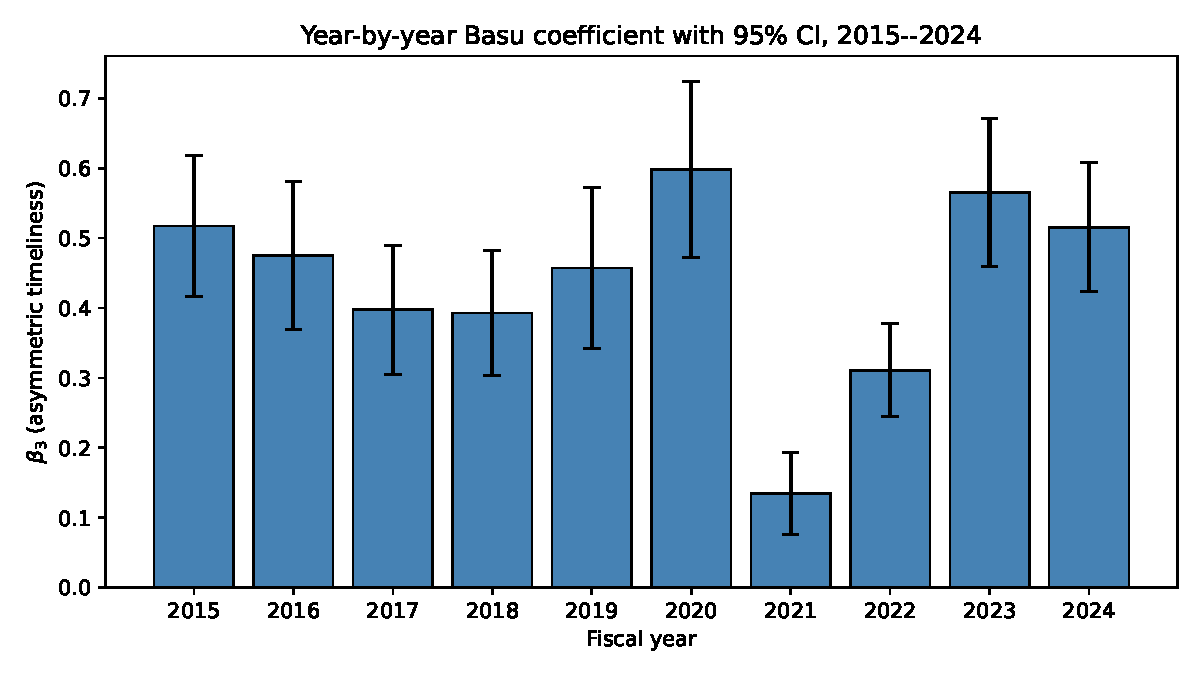
\includegraphics[width=0.85\linewidth]{../output/figures/fig1_beta3_yearly.pdf}
  \caption{Year-by-year estimate of the asymmetric-timeliness coefficient
    $\beta_{3}$ from equation~\eqref{eq:basu}, with 95\% confidence
    intervals based on firm-clustered standard errors.}
  \label{fig:beta3}
\end{figure}

\end{document}
